\parindent=1.5em
Esta memoria está enfocada a abordar un problema financiero, relacionado con las series financieras de alta frecuencia y una forma particular
de poder realizar pronósticos. Se pretende abordar esta problemática con metodologías computacionales, aplicando algunos conceptos matemáticos
útiles para esta área.

La naturaleza del problema es de carácter financiero, por lo que es necesario introducir algunos conceptos, criterios y términos generales
asociados al área.

Este capítulo tiene como objetivo introducir los conceptos de series de tiempo financierras, sus orígenes y la alta frecuencia.

\section{Mercados Financieros}

El mercado financiero es un espacio con marco institucional que permite poner en contacto a oferentes y demandantes para que efectúen
transacciones financieras. La idea de mercado como foro organizado a la que acuden agentes económicos para efectuar transacciones
queda reducida en el mundo financiero como las bolsas de valores.

El concepto de mercado financiero se utiliza en general para referirse a cualquier mercado organizado en el que se negocien instrumentos financieros
de todo tipo, como por ejemplo, acciones. Además el espacio para generar estas interacciones no necesariamente debe ser físico. Por otro lado el negociar
instrumentos financieros implica a grandes rasgos: intercambiar instrumentos financieros, y definir su precio. Por ende, estos mercados están basados en
las fuerzas de oferta y demanda, ubicando a todos los oferentes en el mismo lugar para facilitarle la búsqueda a los demandantes.

Una de las razones que hace importante este tipo de mercado, es su funcionalidad, ya que permiten por un lado aumentar el capital, siendo esto uno 
de los casos favorables, ya que también hay probabilidades considerables de disminuir el capital; comercio internacional, como en los mercados de 
divisas, por ejemplo Forex; y reunir a quienes necesitan recursos financieros, con los que tienen recursos financieros. Factores claves
que permiten generar los efectos de oferta y demanda.

En este tipo de mercado se definen los siguientes términos:
\begin{itemize}
	\item \emph{Dealer}: Un dealer es un ente presente en los mercados que está dispuestos a comprar o vender.
	\item \emph{Orders}: Operación de compra/venta de activos.
	\item \emph{Bid price}: Precio al cual un \emph{dealer} está dispuesto a comprar.
	\item \emph{Ask price}: Precio al cual un \emph{dealer} está dispuesto a vender.
	\item \emph{Market orders}: instrucción del cliente al dealer, comprar o vender al mejor precio posible dentro de los valores actuales del mercado.
		Esto asegura la realización de la transacción, pero no el precio.
	\item \emph{Limit orders}: es una orden para comprar a un valor máximo (precio determinado), o para vender a un valor mínimo (precio determinado).
		Esto le da al cliente el control sobre el precio al que se ejecuta el comercio, sin embargo, no garantiza la realización de la transacción.
\end{itemize}

El conjunto de \emph{Limit orders} forman los \emph{books} para cierto activo, los cuales proveen información detallada de dicho instrumento. Con estos datos
se forman los llamados bid-ask spreads, que es la diferencia entre el precios cotizados para una venta inmediata (oferta) y una compra inmediata (bid). 
Además se generan los bid-ask qoute, el cual define cotas para el precio de transacción.

\subsection{Mercados bursátiles}
Los mercados bursátiles están clasificados en los mercados de capitales, en donde se negocian activos financieros. Este tipo de mercado provee financiamiento
por medio de la emisión de acciones y permiten luego el intercambio de estas. La aplicación más directa de este tipo de mercados, son las bolsas de valores, cuyo
origen se remonta a finales del siglo XV en las ferias medievales de Europa.

Las bolsas de valores se pueden definir como mercados organizados y especializados, en los que se pueden realizar transacciones de títulos de valores por
medio de intermediarios autorizados. Estas bolsas ofrecen al público y a sus miembros facilidades, mecanismos e instrumentos técnicos que facilitan la negociación
de títulos de valores susceptibles de ofertas públicas, a precios determinados mediante subasta.

La principal función de las Bolsas de Valores implican proporcionar a los participantes información verar, objetiva, completa y permanente de los valores
y las empresas inscritas en la Bolsa, sus emisiones y las operaciones que en ella se realicen, supervisión de actividades.

Las componentes de este sistema son los activos, instituciones financieras cuya misión es contactar demandantes y oferentes en los mercados donde se negocian
los diferentes instrumentos o activos financieros.

Dentro de los estudios de la economía, se habla de que este tipo de mercado es de competencia perfecta, ya que posee características
como: elevado número de compradores y vendedores. La decisión individual de cada uno de ellos ejercerá escasa influencia sobre el mercado global; 
Homogeneidad de los productos, es decir, no existen diferencias entre productos que venden los oferentes; Transparencia del mercado, todos los 
participantes tienen pleno conocimiento de las condiciones generales en que opera el mercado; Libertad de entrada y salida de empresas, todos 
los participantes, cuando lo deseen, podrán entrar o salir del mercado a costos nulos o casi nulos \cite{mankiw2011principles}.

\section{Series de tiempo financiera}

En la vida real, la mayoría de los fenómenos que se estudian secuencialmente, deben
tomar en cuenta la dinámica de los proceso con la finalidad de entenderlos de la mejor manera
posible. Una herramienta muy útil en dicho objetivo es el Análisis de Series de Tiempo. Se
pueden presentar casos de series de tiempo en una multitud de disciplinas como ingeniería,
sociología, economía, finanzas por solo mencionar algunas de ellas.

El propósito fundamental es mostrar las técnicas que permitan hacer inferencias del
proceso en estudio incluyendo su predicción. Esto se logra estableciendo modelos
probabilísticos hipotéticos que representen a los datos; y en consecuencia, se lleva a cabo el
proceso de ajuste que incluye desde la estimación hasta la predicción una vez que se determina
un modelo satisfactorio. Los modelos de series deben considerar la naturaleza del fenómeno y determinar 
los factores que pueden ser incluidos en los modelos.

En particular, el análisis de una series de tiempo financiera se refiere a la teoría y práctica de la valoración 
de activos en el tiempo, es decir, un estudio del precio como función del tiempo.

Es una disciplina muy empírica, pero al igual que la teoría de otros campos científicos es la base para hacer inferencias. 
Hay, sin embargo, una característica clave que distingue el análisis financiero serie de tiempo de otros análisis de series de tiempo. 

Tanto la teoría económica y sus series temporales empíricas contienen un elemento de incertidumbre. Por ejemplo, 
hay varias definiciones de volatilidad de los activos, y para una serie de retornos de las acciones, la volatilidad no es observable directamente.

Las características diferenciadoras han propiciado numerosos trabajos en las áreas de econometría y economía financiera desde los años 70.
Así, en el área financiera las evidencias sobre estructuras ha conducido a la formulación de distintos modelos matemáticos que se estudiarán
en esta memoria.

\section{Cómo se generan y sus características}

Las series de tiempo financieras como se dijo previamente, se basan en el estudio del precio de un activo financiero en el tiempo. Pero existen 
varios tipos de precios que se pueden lograr estudiar. Por un lado están los indicadores que se estudiaron en los primeros estudios formales
en esta área, llamados estudios técnicos, los cuales mostraban información al respecto de los precios: \emph{apertura}, \emph{cierre}, \emph{el más bajo}, 
\emph{el más alto}, \emph{promedio}. Esos datos lógicamente estaban orientados a tomar métricas respecto a la frecuencia \emph{día}, con estos
datos quedaban graficos como el siguiente:

\begin{center}
	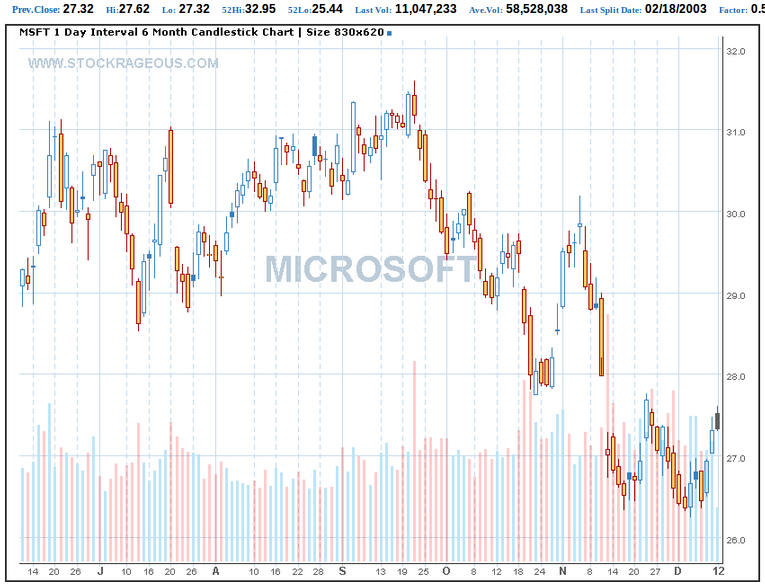
\includegraphics[width=0.6\textwidth]{images/microsoft} \\
	\textbf{Figura 1.} Información de los precios de microsoft en la bolsa.
\end{center}

Esos precios son a nivel diario, sin embargo la data estudiada actualmente corresponde a data \emph{intra diaria}, la cual reside en los valores
específicos en que se compró/vendió algún activo, ya sea acción, divisa, etc. Ese término se conoce como el \emph{last price}, y corresponde
al valor específico con el cual se transó el activo. La forma de como se realiza este evento es básicamente como el que se detalló anteriormente,
es decir, mediante \emph{market} o \emph{limit orders}, por lo que existe una cola de compras/ventas obtenidas mediante los \emph{limit orders} y que cuando
se cumpla la condición asociada (de vender o comprar a cierto precio), se realiza la transacción y se registra dicho \emph{last price}; 
y por otro lado, si se entra a comprar/vender directamente mediante una \emph{market order} también se registra dicho valor. 
Juntando toda esa información entonces, se puede generar una secuencia temporal de los \emph{last prices}.

Ahora bien, estas interacciones antiguamente se realizaban personalmente en las bolsas de comercio, sin embargo con el avance de las tecnologías,
se han implementado distintas plataformas de \emph{trading electrónico}: un método de negociación de valores (como acciones y bonos), divisas o derivados 
financieros por medios electrónicos. Esta tecnología de la información se utiliza para reunir a compradores y vendedores a través de la plataforma de 
comercio electrónico y las redes para crear lugares virtuales del mercado, como por ejemplo: National Association of Securities Dealers Automated 
Quotation (NASDAQ), New York Stock Exchange (NYSE), etc. Estos medios también se conocen como \emph{electronic communications networks} (ECNs).


Las series financieras tienen características singulares en relación a otras series macroeconómicas, como son: 
\begin{itemize}
	\item Frecuencia: la mayor frecuencia en la observación de los datos es mayor que en otro tipo de series de tiempo, llegando incluso
		a unidades de fracciones de segundos.
	\item Heterocedasticidad: ocurre cuando la varianza de las perturbaciones no es constante a lo largo de las observaciones.
		Este factor hace inadecuados los modelos desarrolados para series estcionarias.
	\item No estacionaria: en muchos casos presenta no estacionaridad tanto en la media como la varianza.
		
\end{itemize}

\section{High frequency trading}
